\documentclass[tikz,border=10pt]{standalone}
\usepackage{tikz}
\usetikzlibrary{arrows.meta, positioning}

\begin{document}

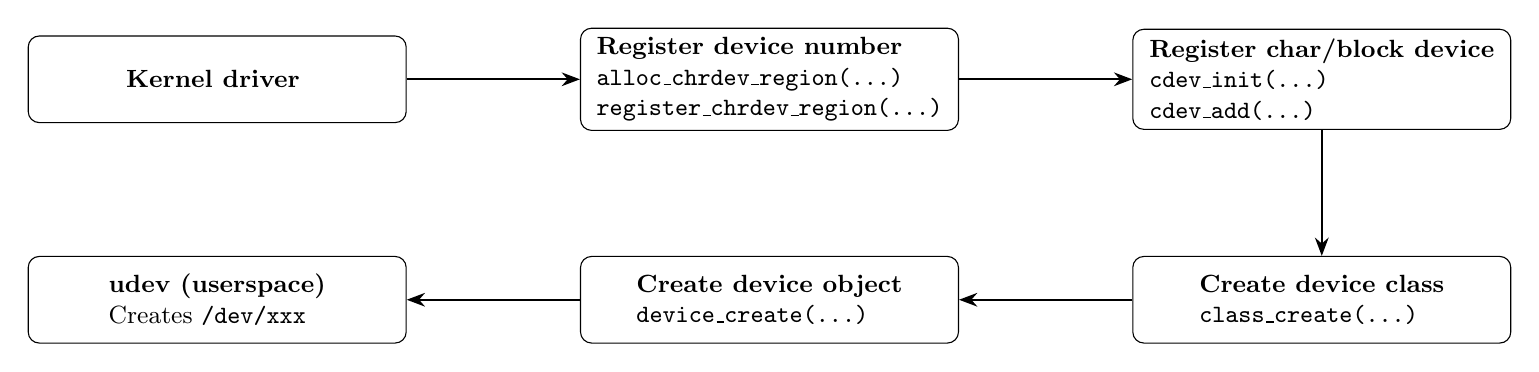
\begin{tikzpicture}[
    box/.style={
        draw,
        rounded corners,
        minimum width=4.8cm,
        minimum height=1.1cm,
        align=left,
        font=\small
    },
    arrow/.style={
        ->,
        thick,
        >=Stealth
    },
    node distance=1.6cm and 2.2cm
]

% ---- Top row (left -> right) ----
\node[box] (driver) {
    \textbf{Kernel driver}
};

\node[box, right=of driver] (alloc) {
    \textbf{Register device number}\\
    \texttt{alloc\_chrdev\_region(...)}\\
    \texttt{register\_chrdev\_region(...)}
};

\node[box, right=of alloc] (cdev) {
    \textbf{Register char/block device}\\
    \texttt{cdev\_init(...)}\\
    \texttt{cdev\_add(...)}
};

% ---- Bottom row (right -> left) ----
\node[box, below=of cdev] (class) {
    \textbf{Create device class}\\
    \texttt{class\_create(...)}
};

\node[box, left=of class] (device) {
    \textbf{Create device object}\\
    \texttt{device\_create(...)}
};

\node[box, left=of device] (udev) {
    \textbf{udev (userspace)}\\
    Creates \texttt{/dev/xxx}
};

% ---- Arrows ----
\draw[arrow] (driver) -- (alloc);
\draw[arrow] (alloc) -- (cdev);

\draw[arrow] (cdev) -- ++(0,-0.9cm) -| (class);

\draw[arrow] (class) -- (device);
\draw[arrow] (device) -- (udev);

\end{tikzpicture}

\end{document}
